\section{Differentiation}

\subsection{Partial, Directional, and Path Derivatives} 

	A simple way to extract derivatives is to fix all of the input components except for one, and treat $f$ as a single-variable function. This results in---for now---a completely separate notion of a derivative. 

	\begin{definition}[Partial Derivative]
		Given function $f: E \subset \mathbb{R}^n \to \mathbb{R}^m$, the $i$th \textbf{partial derivative} of $f$ at $a \in E$ is defined 
		\begin{equation}
			\frac{\partial f}{\partial x_i} \bigg|_{a} \coloneqq \lim_{h \to 0} \frac{f(a + h e_i)}{h} 
		\end{equation}
		where $e_i$ is the $i$th basis vector of $\mathbb{R}^n$. 
	\end{definition}

	Since we are fixing every other parameter except for the $i$th one, we can find the partial derivative by differentiating the function w.r.t. $x_i$ and fixing all other variables. 

	\begin{example}[Partial Derivatives Using Differentiation Rules]
    To find all partial derivatives of the function 
		\begin{equation}
			f(x, y, z) = x \ln(y^2 + z^2), 
		\end{equation}
		We compute 
		\begin{align}
			\frac{\partial f}{\partial x} & = \ln(y^2 + z^2) \\  
			\frac{\partial f}{\partial y} & = x \cdot \frac{1}{y^2+z^2} \cdot (2y) = \frac{2xy}{y^2+z^2} \\
			\frac{\partial f}{\partial z} & = x \cdot \frac{1}{y^2+z^2} \cdot (2z) = \frac{2xz}{y^2+z^2}
		\end{align}
	\end{example}

	\begin{example}[Partial Derivatives Using Limit Definition]
		Let 
		\begin{equation}
			f(x, y) =
			\begin{cases}
				\dfrac{xy}{x^2+y^2} & (x,y) \neq (0,0), \\
				0 & (x,y) = (0,0).
			\end{cases}
		\end{equation}
		We compute the partial derivatives $f_x(0,0)$ and $f_y(0,0)$ using the limit definition.

		First, for the partial derivative with respect to $x$, we have
		\begin{align}
			f_x(0,0)
			&=
			\lim_{h\to 0}
			\frac{f(h,0)-f(0,0)}{h} \\
			&=
			\lim_{h\to 0}
			\frac{\dfrac{h(0)}{h^2+0^2}-0}{h} \\
			&=
			\lim_{h\to 0}
			\frac{0}{h} \\
			&= 0.
		\end{align}

		Similarly, for the partial derivative with respect to $y$, we have
		\begin{align}
			f_y(0,0)
			&=
			\lim_{h\to 0}
			\frac{f(0,h)-f(0,0)}{h} \\
			&=
			\lim_{h\to 0}
			\frac{\dfrac{0(h)}{0^2+h^2}-0}{h} \\
			&=
			\lim_{h\to 0}
			\frac{0}{h} \\
			&= 0.
		\end{align}

		Therefore,
		\begin{equation}
			f_x(0,0)=0
			\qquad \text{and} \qquad
			f_y(0,0)=0.
		\end{equation}

		Note that even though the limit of $f(x,y)$ as $(x,y)\to(0,0)$ does not exist, the partial derivatives at $(0,0)$ still exist.
	\end{example}

	The partial derivative looks at the function as it is approaching $a$ along an axis, but we can consider any direction in the domain. 

	\begin{definition}[Directional Derivative]
		Given function $f: E \subset \mathbb{R}^n \to \mathbb{R}^m$, the \textbf{directional derivative} of $f$ at $a \in E$ in direction $u \in \mathbb{R}^n$ is defined 
		\begin{equation}
			D_v f(a) \coloneqq \lim_{h \to 0} \frac{f(a + hu)}{h} 
		\end{equation}
	\end{definition}

	It should be obvious that if all directional derivatives exist, then the partials exist (since we can just set the directional vectors to be the unit vectors). 

	When computing directional derivatives, it is convenient to normalize the directional vector $\mathbf{v}$ to be unit length so that it coincides with the partial derivatives. We don't technically need to set $||\mathbf{v}|| = 1$, but if we have two vectors $\mathbf{v}$ and a scaled $c \mathbf{v}$, then the directional derivatives will also be scaled ($\nabla_{c \mathbf{v}} f (a) = c \nabla_{\mathbf{v}} f (a)$), so we will only work with unit directional vectors. Some say that this restriction is undesirable, since it loses the linearity of the function $\mathbf{v} \mapsto \partial_\mathbf{v} f (a)$. 

	\begin{example}
		Let
		\begin{equation}
			f(x,y) = x^2y + 4y^2.
		\end{equation}
		We compute the directional derivative of $f$ at the point $(2,1)$ in the direction of the vector
		\[
			v=(1,1).
		\]
		First, we normalize $v$. Since
		\begin{equation}
			\|v\| = \sqrt{1^2+1^2} = \sqrt{2},
		\end{equation}
		the unit direction vector is
		\begin{equation}
			u = \frac{v}{\|v\|}
			=
			\left(\frac{1}{\sqrt{2}}, \frac{1}{\sqrt{2}}\right).
		\end{equation}

		By the limit definition of the directional derivative,
		\begin{align}
			D_u f(2,1)
			&=
			\lim_{h\to 0}
			\frac{f\big((2,1)+hu\big)-f(2,1)}{h} \\
			&=
			\lim_{h\to 0}
			\frac{
				f\left(2+\frac{h}{\sqrt{2}}, 1+\frac{h}{\sqrt{2}}\right)
				- f(2,1)
			}{h}.
		\end{align}
		Now,
		\begin{equation}
			f(2,1) = 2^2(1)+4(1)^2 = 8.
		\end{equation}
		Also,
		\begin{align}
			f\left(2+\frac{h}{\sqrt{2}}, 1+\frac{h}{\sqrt{2}}\right)
			&=
			\left(2+\frac{h}{\sqrt{2}}\right)^2
			\left(1+\frac{h}{\sqrt{2}}\right)
			+
			4\left(1+\frac{h}{\sqrt{2}}\right)^2 \\
			&=
			8 + \frac{16h}{\sqrt{2}} + \frac{9h^2}{2}
			+ \frac{h^3}{2\sqrt{2}}.
		\end{align}
		Therefore,
		\begin{align}
			D_u f(2,1)
			&=
			\lim_{h\to 0}
			\frac{
				8 + \frac{16h}{\sqrt{2}} + \frac{9h^2}{2}
				+ \frac{h^3}{2\sqrt{2}} - 8
			}{h} \\
			&=
			\lim_{h\to 0}
			\left(
				\frac{16}{\sqrt{2}} + \frac{9h}{2}
				+ \frac{h^2}{2\sqrt{2}}
			\right) \\
			&=
			\frac{16}{\sqrt{2}} \\
			&=
			8\sqrt{2}.
		\end{align}
	\end{example}

	\begin{example}
		Let
		\begin{equation}
			f(x,y,z,w) = x^2y + z\cos(w).
		\end{equation}
		We compute the directional derivative of $f$ at the point $(1,2,0,0)$ in the direction of the vector
		\[
			v=(1,1,1,1).
		\]
		First, we normalize $v$. Since
		\begin{equation}
			\|v\|
			=
			\sqrt{1^2+1^2+1^2+1^2}
			=
			2,
		\end{equation}
		the unit direction vector is
		\begin{equation}
			u = \frac{v}{\|v\|}
			=
			\left(\frac{1}{2}, \frac{1}{2}, \frac{1}{2}, \frac{1}{2}\right).
		\end{equation}

		By the limit definition of the directional derivative,
		\begin{align}
			D_u f(1,2,0,0)
			&=
			\lim_{h\to 0}
			\frac{f\big((1,2,0,0)+hu\big)-f(1,2,0,0)}{h} \\
			&=
			\lim_{h\to 0}
			\frac{
				f\left(1+\frac{h}{2}, 2+\frac{h}{2}, \frac{h}{2}, \frac{h}{2}\right)
				- f(1,2,0,0)
			}{h}.
		\end{align}
		Now,
		\begin{equation}
			f(1,2,0,0) = 1^2(2) + 0\cos(0) = 2.
		\end{equation}
		Also,
		\begin{align}
			f\left(1+\frac{h}{2}, 2+\frac{h}{2}, \frac{h}{2}, \frac{h}{2}\right)
			&=
			\left(1+\frac{h}{2}\right)^2
			\left(2+\frac{h}{2}\right)
			+
			\frac{h}{2}\cos\left(\frac{h}{2}\right) \\
			&=
			\left(1+h+\frac{h^2}{4}\right)
			\left(2+\frac{h}{2}\right)
			+
			\frac{h}{2}\cos\left(\frac{h}{2}\right) \\
			&=
			2 + \frac{5h}{2} + h^2 + \frac{h^3}{8}
			+
			\frac{h}{2}\cos\left(\frac{h}{2}\right).
		\end{align}
		Therefore,
		\begin{align}
			D_u f(1,2,0,0)
			&=
			\lim_{h\to 0}
			\frac{
				2 + \frac{5h}{2} + h^2 + \frac{h^3}{8}
				+
				\frac{h}{2}\cos\left(\frac{h}{2}\right)
				- 2
			}{h} \\
			&=
			\lim_{h\to 0}
			\left(
				\frac{5}{2}
				+
				h
				+
				\frac{h^2}{8}
				+
				\frac{1}{2}\cos\left(\frac{h}{2}\right)
			\right) \\
			&=
			\frac{5}{2} + \frac{1}{2} \\
			&=
			3.
		\end{align}
	\end{example}

	But be careful! The existence of partials does not imply the existence of all directional derivatives! 

  \begin{example}[Existence of Partials $\centernot \implies$ Existence of Directional Derivatives]
    Consider the function 
    \[f(x_1, x_2) = \begin{cases} 
    \frac{x_1 x_2}{x_1^2 + x_2^2} & \text{ if } (x_1, x_2) \neq (0, 0) \\
    0 & \text{ if } (x_1, x_2) = (0, 0) 
    \end{cases}\]
    The partial derivatives exist everywhere. Away from the origin we can simply compute 
    \begin{align*}
        \frac{\partial f}{\partial x_1} = \frac{x_2 (x_1^2 + x_2^2) - x_1 x_2 \cdot 2x_1}{(x_1^2 + x_2^2)^2} = \frac{- x_1^2 x_2 + x_2^3}{(x_1^2 + x_2^2)^2} \\
        \frac{\partial f}{\partial x_2} = \frac{x_1 (x_1^2 + x_2^2) - x_1 x_2 \cdot 2 x_2}{(x_1^2 + x_2^2)^2} = \frac{x_1^3 - x_1 x_2^2}{(x_1^2 + x_2^2)^2}
    \end{align*}
    As for the partials at the origin, we must compute using the limit rule. 
    \begin{align*}
        \partial_{x_1} f (\mathbf{0}) & = \lim_{h \rightarrow 0} \frac{f(\mathbf{0} + h \mathbf{e}_1) - f(\mathbf{0})}{h} = \lim_{h \rightarrow 0} \frac{f(h, 0)}{h} = 0  \\
        \partial_{x_2} f (\mathbf{0}) & = \lim_{h \rightarrow 0} \frac{f(\mathbf{0} + h \mathbf{e}_2) - f(\mathbf{0})}{h} = \lim_{h \rightarrow 0} \frac{f(0, h)}{h} = 0
    \end{align*}
    However, the directional derivative taken in direction $\mathbf{v} = (1, 1)$ gives 
    \begin{align*}
        \nabla_{(1, 1)} f (0, 0) & = \lim_{h \rightarrow 0} \frac{f(\mathbf{0} + h (1, 1)) - f(\mathbf{0})}{h} \\
        & = \lim_{h \rightarrow 0} \frac{f(h, h)}{h} \\
        & = \lim_{h \rightarrow 0} \frac{1}{2h} 
    \end{align*}
    which does not have a limit as $h \rightarrow 0$. To visualize this, let's look at the values of $f$ along various lines in $\mathbb{R}^2$. 
    \begin{enumerate}
        \item $f = 0$ at the line $x_1 = 0$ and $x_2 = 0$, which is why the partials are $0$. 
        \item $f = \frac{1}{2}$ at the line where $x_1 = x_2$, except for the point $(0, 0)$, where $f = 0$, which is why the limit in the direction doesn't exist. 
    \end{enumerate}
  \end{example}

	\begin{definition}[Path Derivative]
		Let $f: E \subset \mathbb{R}^n \to \mathbb{R}^m$, $a \in E$, and $p: \mathbb{R} \to \mathbb{R}^n$ be a path function where $p(t_0) = a$. Then, the \textbf{path derivative} of $f$ at $a$ with respect to path $p$ is defined  
		\begin{equation}
			D_p f(a) \coloneqq \lim_{t \to t_0} \frac{f(p(t)) - f(p(t_0))}{h} 
		\end{equation}
	\end{definition}

	\begin{example}
		Let
		\begin{equation}
			f(x,y) = x^2+y,
		\end{equation}
		and let
		\begin{equation}
			p(t) = (1+t, 1+t^2).
		\end{equation}
		Since
		\begin{equation}
			p(0) = (1,1),
		\end{equation}
		we compute the path derivative of $f$ at $a=(1,1)$ with respect to the path $p$.

		By the definition of the path derivative,
		\begin{align}
			D_p f(1,1)
			&=
			\lim_{t\to 0}
			\frac{f(p(t))-f(p(0))}{t-0} \\
			&=
			\lim_{t\to 0}
			\frac{f(1+t,1+t^2)-f(1,1)}{t}.
		\end{align}
		Now,
		\begin{equation}
			f(1,1) = 1^2+1 = 2,
		\end{equation}
		and
		\begin{align}
			f(1+t,1+t^2)
			&=
			(1+t)^2 + (1+t^2) \\
			&=
			1+2t+t^2+1+t^2 \\
			&=
			2+2t+2t^2.
		\end{align}
		Therefore,
		\begin{align}
			D_p f(1,1)
			&=
			\lim_{t\to 0}
			\frac{2+2t+2t^2-2}{t} \\
			&=
			\lim_{t\to 0}
			\frac{2t+2t^2}{t} \\
			&=
			\lim_{t\to 0}
			(2+2t) \\
			&=
			2.
		\end{align}
	\end{example}

	\begin{example}
		Let
		\begin{equation}
			f(x,y) = (xy, x^2-y),
		\end{equation}
		and let
		\begin{equation}
			p(t) = (\cos t, \sin t).
		\end{equation}
		Since
		\begin{equation}
			p(0) = (1,0),
		\end{equation}
		we compute the path derivative of $f$ at $a=(1,0)$ with respect to the path $p$.

		By the definition of the path derivative,
		\begin{align}
			D_p f(1,0)
			&=
			\lim_{t\to 0}
			\frac{f(p(t))-f(p(0))}{t-0} \\
			&=
			\lim_{t\to 0}
			\frac{f(\cos t,\sin t)-f(1,0)}{t}.
		\end{align}
		Now,
		\begin{equation}
			f(1,0) = (0,1),
		\end{equation}
		and
		\begin{align}
			f(\cos t,\sin t)
			&=
			\big(\cos t \sin t, \cos^2 t - \sin t\big).
		\end{align}
		Therefore,
		\begin{align}
			D_p f(1,0)
			&=
			\lim_{t\to 0}
			\frac{
				\big(\cos t \sin t, \cos^2 t - \sin t\big) - (0,1)
			}{t} \\
			&=
			\lim_{t\to 0}
			\left(
				\frac{\cos t \sin t}{t},
				\frac{\cos^2 t - \sin t - 1}{t}
			\right).
		\end{align}
		We compute each component separately. For the first component,
		\begin{align}
			\lim_{t\to 0}
			\frac{\cos t \sin t}{t}
			&=
			\lim_{t\to 0}
			\cos t \cdot \frac{\sin t}{t} \\
			&=
			1.
		\end{align}
		For the second component,
		\begin{align}
			\lim_{t\to 0}
			\frac{\cos^2 t - \sin t - 1}{t}
			&=
			\lim_{t\to 0}
			\left(
				\frac{\cos^2 t - 1}{t}
				-
				\frac{\sin t}{t}
			\right) \\
			&=
			\lim_{t\to 0}
			\left(
				\frac{-\sin^2 t}{t}
				-
				\frac{\sin t}{t}
			\right) \\
			&=
			0 - 1 \\
			&=
			-1.
		\end{align}
		Hence,
		\begin{equation}
			D_p f(1,0) = (1,-1).
		\end{equation}
	\end{example}

\subsection{Total Derivatives}

  \begin{definition}[Total/Frechet Derivative]
		\label{def:derivative}
		Let $f: E \subset \mathbb{R}^n \to \mathbb{R}^m$ and $a \in E$. $f$ is \textbf{differentiable} at $a$ if it satisfies either of the equivalent conditions. 

		\begin{enumerate}
			\item \textit{Linear Approximation}. There exists a linear map $Df_a: \mathbb{R}^n \longrightarrow \mathbb{R}^m$\footnote{Note that when $m = 1$, then $Df_a$ is a linear functional, i.e. a dual vector.} such that 
				\begin{equation}
					\lim_{h \to 0} \frac{\| f(a + h) - f(a) - Df_a h \|}{\| h \|} = 0 
				\end{equation} 

			\item \textit{Fundamental Increment Lemma}. There exists a linear map $Df_a: \mathbb{R}^n \to \mathbb{R}^m$ and a function $\Phi: \mathbb{R}^n \to \mathbb{R}^m$ defined for sufficiently small nonzero $h \in \mathbb{R}^n$ such that 
				\begin{equation}
					f(a + h) = f(a) + Df_a h + \Phi(h) \|h\|, \qquad \lim_{h \to 0} \Phi(h) = 0
				\end{equation}
		\end{enumerate}
		If such a map $D f_a$ exists, then it is unique, and we call this the \textbf{total derivative}---or \textbf{Frechet derivative}---of $f$ at $a$. 
  \end{definition}
  \begin{proof}
    The only claim to prove is uniqueness if defined. 
  \end{proof} 

  The reason we want $E$ to be open is that we require that $x + h$ to also be in $D$ for sufficiently small $h$, and we can guarantee this since an $\epsilon$-ball around $x$ is guaranteed to be in $E$. 


  Therefore, we have 4 separate notions of derivatives. A natural question to ask is whether the existence of one derivative implies the existence of another. 

  \begin{theorem}[Differentiability $\implies$ Existence of All Directionals] 
		If $f: E \subset \mathbb{R}^n \to \mathbb{R}^m$ is differentiable at $a \in E$, then all of its directional derivatives exist. Furthermore, given direction vector $u \in \mathbb{R}^n$, 
		\begin{equation}
		  D_u f_a = Df_a (u)
		\end{equation}
		That is, we can compute the directional derivative by plugging in the direction vector into the linear map $Df_a$.  
  \end{theorem} 
	\begin{proof}
		The partial derivative equals the image of the basis vector 
		\begin{equation}
			\frac{\partial f_j}{\partial x_i} = (D f_x e_i)_j
		\end{equation}
		Therefore by linearity, it holds for directional derivatives. 
	\end{proof}

  Therefore, we know that differentiability (i.e. existence of the total derivative) is the strongest. If this is the case, then the partial and directional derivatives exist. Furthermore, since our vector spaces come with a basis, we can realize $Df_x$ in a matrix form. 

  \begin{definition}[Jacobian]
    Given $f: E \subset \mathbb{R}^n \to \mathbb{R}^m$ differentiable at $x$, the \textbf{Jacobian} of $f$ at $x$ is the matrix realization of the total derivative, with entries being precisely the partial derivatives. 
		\begin{equation}
			Jf_a = \begin{pmatrix} 
				\frac{\partial f_1}{\partial x_1} & \ldots & \frac{\partial f_1}{\partial x_n} \\ 
				\vdots & \ddots & \vdots \\ 
				\frac{\partial f_m}{\partial x_1} & \ldots & \frac{\partial f_m}{\partial x_n}
			\end{pmatrix}
		\end{equation}
  \end{definition} 
	\begin{proof}
	  Immediate result by looking at how it acts on the basis vectors. 
	\end{proof}

  Analogous to the univariate case, a nice way to visualize the derivative is by looking at the tangent \textit{plane}. In general, we have an \textit{affine hyperplane}. Define this here. Unfortunately, the only types of functions that we can meaningful visualize are those mapping $f: \mathbb{R}^2 \to \mathbb{R}$. 

	\begin{definition}[Tangent Hyperplane]
		If $f: E \subset \mathbb{R}^n \to \mathbb{R}$ is differentiable at $a\in\mathbb{R}^n$, then the affine hyperplane tangent to the graph of $f$ at $(a,f(a))$ is the set
		\begin{equation}
			P = \{(x, f(x) \colon z = f(a) + Df_a(x-a)\}.
		\end{equation}
	\end{definition}

	\begin{figure}[H]
		\centering
		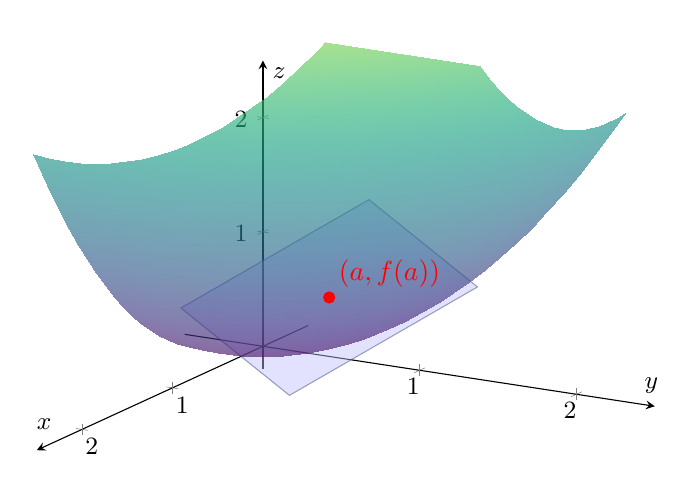
\begin{tikzpicture}
			\begin{axis}[
				view={120}{25},
				axis lines=center,
				xlabel={$x$},
				ylabel={$y$},
				zlabel={$z$},
				xmin=-0.5, xmax=2.5,
				ymin=-0.5, ymax=2.5,
				zmin=-0.2, zmax=2.5,
				domain=-0.2:2.2,
				y domain=-0.2:2.2,
				samples=25,
				samples y=25,
				colormap/viridis,
				width=11cm,
				height=8cm,
				grid=major,
				tick label style={font=\small},
				label style={font=\small},
			]

				% Tangent plane at (1,1)
				% f(x,y) = (x^2+y^2)/2
				% f(1,1)=1, f_x(1,1)=1, f_y(1,1)=1
				% tangent plane: z = 1 + (x-1) + (y-1) = x+y-1
				\addplot3[
					surf,
					domain=0.4:1.6,
					y domain=0.4:1.6,
					samples=2,
					samples y=2,
					opacity=0.45,
					draw=blue,
					fill=blue!25,
				]
				{x + y - 1};

				% Surface: z = (x^2 + y^2)/2
				\addplot3[
					surf,
					opacity=0.65,
					shader=interp,
				]
				{0.5*(x^2 + y^2)};

				% Point of tangency
				\addplot3[
					only marks,
					mark=*,
					mark size=2pt,
					color=red,
				]
				coordinates {(1,1,1)};

				% Label for point
				\node[red, above right] at (axis cs:1,1,1) {$(a,f(a))$};
			\end{axis}
		\end{tikzpicture}
		\caption{The tangent plane to the surface $z=f(x,y)$ at the point $(a,f(a))$. Here $f(x,y)=\frac{x^2+y^2}{2}$ and $a=(1,1)$, so the tangent plane is $z=x+y-1$.}
		\label{fig:tangent_plane}
	\end{figure}

  So, to prove that a function $f: \mathbb{R}^n \longrightarrow \mathbb{R}$ is differentiable at $a$, and if so, what its total derivative is, there are essentially two steps. 
  \begin{enumerate}
    \item We find a candidate for $M$ by evaluating the partials. 
    \begin{equation}
      M = \begin{pmatrix} \partial_{x_1} f(a) & \partial_{x_2} f(a) & \ldots & \partial_{x_n} f(a) \end{pmatrix}
    \end{equation}
    \item We check to see if the limit is true. 
    \begin{equation}
      \lim_{\mathbf{h} \rightarrow \mathbf{0}} \frac{f(a + \mathbf{h}) - f(a) - M \mathbf{h}}{||\mathbf{h}||} = 0
    \end{equation}
    If it is, then $D f_a = M$, and the "tangent plane" of $f$ at $a$ is defined by the equation $y = f(a) + M \mathbf{h}$. 
  \end{enumerate}

  \begin{example}[Computing Total Derivative]
    The function $f(x_1, x_2) = x_1^2 + x_2^2$ is differentiable at $(1, 1)$. We let $M = \big(\partial_{x_1} f(1, 1), \partial_{x_2} f(1, 1) \big) = \big(2, 2\big)$ and see that 
    \begin{align}
      \lim_{\mathbf{h} \rightarrow \mathbf{0}} \frac{f(a + \mathbf{h}) - f(a) - M \mathbf{h}}{||\mathbf{h}||} & = \lim_{\mathbf{h} \rightarrow \mathbf{0}} \frac{f(1 + h_1, 1 + h_2) - f(1, 1) - 2 h_1 - 2 h_2}{\sqrt{h_1^2 + h_2^2}} \\
      & = \lim_{\mathbf{h} \rightarrow \mathbf{0}} \frac{(1 + h_1)^2 + (1 + h_2)^2 - 2 - 2 h_1 - 2 h_2}{\sqrt{h_1^2 + h_2^2}} \\
      & = \lim_{\mathbf{h} \rightarrow \mathbf{0}} \sqrt{h_1^2 + h_2^2} = 0
    \end{align}
    So, $D f (1, 1) = (2, 2)$. 
  \end{example}

  \begin{example}[Computing Tangent Plane]
    Let us find the equation of the tangent plane to $f(x, y) = \ln(2x + y)$ at $(-1, 3)$. Our total derivative, if it exists, is the covector of partials
    \begin{equation}
      D f = \begin{pmatrix} \frac{\partial f}{\partial x} & \frac{\partial f}{\partial y} \end{pmatrix} = \begin{pmatrix} \frac{2}{2x + y} & \frac{1}{2x + y} \end{pmatrix}
    \end{equation}
    which is indeed continuous at a neighborhood of $(-1, 3)$ (in fact, in every neighborhood not containing $\mathbf{0}$). By continuity of partials, $f$ is differentiable at $(-1, 3)$, with $D f_{(-1, 3)} = (2, 1)$. The equation of the plane is then 
    \begin{equation}
      z = f(-1, 3) + D f_{(-1, 3)} \begin{pmatrix} x + 1\\ y - 3 \end{pmatrix} = 2(x + 1) + 1 (y - 3) \implies z = 2x + y - 1
    \end{equation}
  \end{example}

  However, the converse is not true for either statements. You cannot just evaluate all the partial derivatives and assume that the total derivative exists!  

	\begin{example}[Partial Derivatives Exist, but Not Differentiable]
		Consider the function $f: \mathbb{R}^2 \to \mathbb{R}$ defined by:
		\begin{equation}
		  f(x, y) = \begin{cases} \frac{xy}{x^2 + y^2} & (x, y) \neq (0, 0) \\ 0 & (x, y) = (0, 0) \end{cases} 
		\end{equation}
		At the origin $(0, 0)$, the partial derivatives are:
		\begin{equation}
			\frac{\partial f}{\partial x}(0, 0) = \lim_{h \to 0} \frac{f(h, 0) - f(0, 0)}{h} = \lim_{h \to 0} \frac{0 - 0}{h} = 0. 
		\end{equation}

		Similarly, $\frac{\partial f}{\partial y}(0, 0) = 0$. Both partial derivatives exist. However, the total derivative \textbf{cannot} exist because the function is not continuous at $(0, 0)$. As we saw in the limits section, approaching along $y=x$ gives a limit of $1/2$, while the function value is $0$. A fundamental property of differentiability is that it implies continuity; therefore, $f$ is not differentiable at the origin.

		\begin{figure}[H]
			\centering
			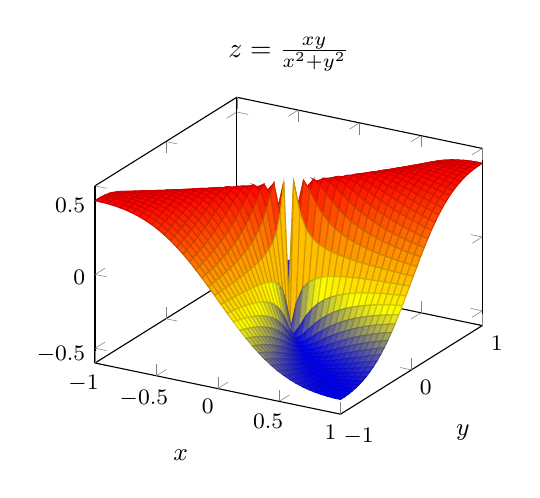
\begin{tikzpicture}
				\begin{axis}[
					title={$z = \frac{xy}{x^2 + y^2}$},
					xlabel=$x$, ylabel=$y$,
					small,
					view={30}{30},
				]
				\addplot3[
					surf,
					domain=-1:1,
					domain y=-1:1,
					samples=40,
				] {x*y / (x^2 + y^2)};
				\end{axis}
			\end{tikzpicture}
			\caption{A function where partial derivatives exist at the origin, but the surface is ``torn'' there.}
		\end{figure}
	\end{example}

	\begin{example}[All Directional Derivatives Exist, but Not Differentiable]
		Consider $f(x, y) = \begin{cases} \frac{x^2 y}{x^4 + y^2} & (x, y) \neq (0, 0) \\ 0 & (x, y) = (0, 0) \end{cases}$. For any direction $\mathbf{u} = (u_1, u_2)$, the directional derivative at the origin exists and is given by $D_{\mathbf{u}}f(0,0) = \frac{u_1^2}{u_2}$ (if $u_2 \neq 0$) or $0$ (if $u_2 = 0$). 
		
		Despite having directional derivatives in every single direction, the total derivative does not exist. First, $f$ is not continuous at the origin (approaching along $y=x^2$ gives $1/2 \neq 0$). Second, even if it were continuous, the total derivative requires that the linear map $Df(a)$ approximates the function well in \textit{every} manner of approach, not just along straight lines. Here, the ``peak'' of the function follows the parabola $y=x^2$, which escapes the linear approximation provided by the directional derivatives.

		\begin{figure}[H]
			\centering
			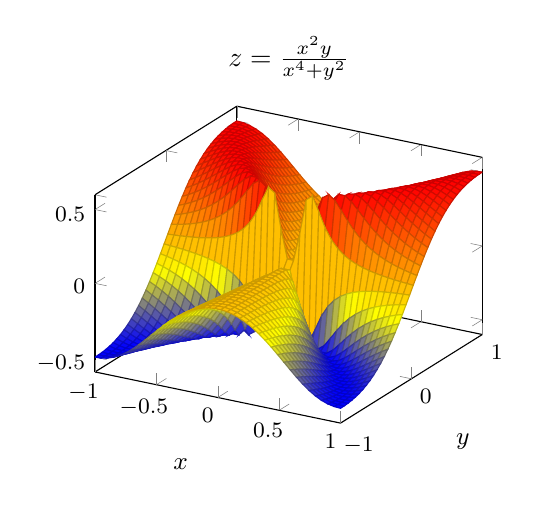
\begin{tikzpicture}
				\begin{axis}[
					title={$z = \frac{x^2 y}{x^4 + y^2}$},
					xlabel=$x$, ylabel=$y$,
					small,
					view={30}{30},
				]
				\addplot3[
					surf,
					domain=-1:1,
					domain y=-1:1,
					samples=40,
				] {x^2*y / (x^4 + y^2)};
				\end{axis}
			\end{tikzpicture}
			\caption{A function where all directional derivatives exist at the origin, yet the surface is non-differentiable.}
		\end{figure}
	\end{example}

\subsection{Rules of Differentiation}

  Just like single variable calculus, the total derivative behaves in predictable ways: it is linear, product/quotient rules, and the chain rule. 

  \begin{theorem}[Linearity of Total Derivatives]
    Let $f, g: E \subset \mathbb{R}^n \longrightarrow \mathbb{R}^m$ be differentiable at $a \in E$. Then, the total derivative at $a$ is linear w.r.t. the input functions. 
    \begin{enumerate}
      \item \textit{Addition}. $D (f + g)_a = D f_a + D g_a$ 
      \item \textit{Scalar Multiplication}. $D (c f)_a = c D f_a$ 
    \end{enumerate}
  \end{theorem}

  Note that for the product and quotient rules, our scope is only for scalar valued functions since products and quotients aren't defined over codomains that are vector spaces. 

  \begin{theorem}[Product Rule]
    Let $f, g: E \subset \mathbb{R}^n \longrightarrow \mathbb{R}$ be differentiable at $a$. Then, 
    \begin{equation}
			D (f g)_a = D f_a g(a) + f(a) D g_a
    \end{equation}
  \end{theorem}

  \begin{theorem}[Quotient Rule]
		Let $f, g: E \subset \mathbb{R}^n \longrightarrow \mathbb{R}$ be differentiable at $a$ with $g(a) \neq 0$. Then, 
		\begin{equation}
			D \Big( \frac{f}{g} \Big)_a = \frac{D f_a g(a) - f(a) D g_a}{g(a)^2}
		\end{equation}
  \end{theorem}

  \begin{theorem}[Chain Rule]
		Let $f: E \subset \mathbb{R}^n \longrightarrow \mathbb{R}^m$ be differentiable at $a \in E$ and $g: E^\prime \subset \mathbb{R}^m \longrightarrow \mathbb{R}^p$ be differentiable at $g(a) \in E^\prime$. Then, $g \circ f$ is differentiable at $a$, and 
		\begin{equation}
			D (g \circ f)_a = D g_{f(a)} \circ D f_a
		\end{equation}
  \end{theorem}

  Therefore, given the composition of function $f \circ g$, we have two methods of finding the derivative matrix of $f \circ g$ at point $x_0$. First is to explicitly compute $f \circ g$ and find its $m \times p$ derivative matrix $D (f \circ g)$, and plug in $a$ to get $D(f\circ g)_a$. The second way is to use the chain rule to find the individual total derivatives $D f_{g(a)}$ and $D g_a$, and multiply them together. 

\subsection{Continuously Differentiable Functions}

  An even stronger condition beyond differentiability is continuous partials, and we often prove continuity of partials to prove differentiability. 

  \begin{theorem}[Continuous Partials $\implies$ Differentiability]
    Given a function $f: E \subset \mathbb{R}^n \longrightarrow \mathbb{R}$ and a point $a \in E$, if all the partials $\partial_{x_i} f$ exist and are continuous at $a$, then $f$ is differentiable at $a$. 

		\begin{figure}[H]
			\centering
			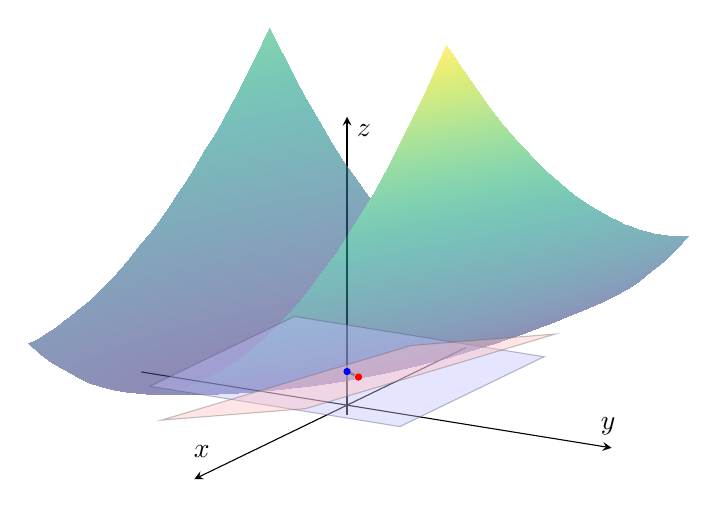
\begin{tikzpicture}
				\begin{axis}[
					view={120}{27},
					axis lines=center,
					xmin=-1.4, xmax=1.8,
					ymin=-1.4, ymax=1.8,
					zmin=-0.1, zmax=3.0,
					domain=-1.25:1.6,
					y domain=-1.25:1.6,
					samples=35,
					samples y=35,
					width=11cm,
					height=8cm,
					grid=none,
					ticks=none,
					xlabel={$x$},
					ylabel={$y$},
					zlabel={$z$},
					clip=false,
				]

					% Surface:
					% f(x,y) = 0.25x^2 + 0.85y^2 + 0.65xy + 0.35
					\addplot3[
						surf,
						opacity=0.60,
						shader=interp,
						colormap/viridis,
					]
					{0.25*x^2 + 0.85*y^2 + 0.65*x*y + 0.35};

					% First tangent plane at a = (0,0)
					% Tangent plane: z = 0.35
					\addplot3[
						surf,
						domain=-0.85:0.85,
						y domain=-0.85:0.85,
						samples=2,
						samples y=2,
						opacity=0.40,
						draw=blue,
						fill=blue!25,
					]
					{0.35};

					% Point of tangency for first plane
					\addplot3[
						only marks,
						mark=*,
						mark size=1.1pt,
						color=blue,
					]
					coordinates {(0,0,0.35)};

					% Second tangent plane at b = (0.35,0.28)
					%
					% f(0.35,0.28) = 0.510965
					% f_x(0.35,0.28) = 0.357
					% f_y(0.35,0.28) = 0.7035
					%
					% Tangent plane:
					% z = 0.510965 + 0.357(x-0.35) + 0.7035(y-0.28)
					\addplot3[
						surf,
						domain=-0.50:1.20,
						y domain=-0.57:1.13,
						samples=2,
						samples y=2,
						opacity=0.40,
						draw=red,
						fill=red!25,
					]
					{0.510965 + 0.357*(x-0.35) + 0.7035*(y-0.28)};

					% Point of tangency for second plane
					\addplot3[
						only marks,
						mark=*,
						mark size=1.1pt,
						color=red,
					]
					coordinates {(0.35,0.28,0.510965)};

					% Dashed line connecting the nearby points
					\addplot3[
						dashed,
						gray,
						thick,
					]
					coordinates {(0,0,0.35) (0.35,0.28,0.510965)};

				\end{axis}
			\end{tikzpicture}
			\caption{We can also visualize this theorem. Since the partials are continuous, then the tangent subspace, which is determined by the span of the tangent vectors determined by the partials, also changes continuously, and therefore the total derivative within a neighborhood of $a$ exists. }
			\label{fig:perturbed_tangent_planes}
		\end{figure}
  \end{theorem}

	While continuous partial derivatives guarantee differentiability, the converse is not true. A function can be differentiable even if its partial derivatives are not continuous. However, if they are not continuous, we cannot use the previous theorem to determine differentiability and must revert to the definition.

	\begin{example}[Non-Continuous Partials and Not Differentiable]
		Recall $f(x, y) = \begin{cases} \frac{xy}{x^2 + y^2} & (x, y) \neq (0, 0) \\ 0 & (x, y) = (0, 0) \end{cases}$.
		The partial derivative $\frac{\partial f}{\partial x}$ for $(x, y) \neq (0, 0)$ is:
		\[ \frac{\partial f}{\partial x} = \frac{y(x^2 + y^2) - xy(2x)}{(x^2 + y^2)^2} = \frac{y^3 - x^2 y}{(x^2 + y^2)^2}. \]
		At the origin, we found $\frac{\partial f}{\partial x}(0, 0) = 0$. However, $\lim_{(x, y) \to (0, 0)} \frac{y^3 - x^2 y}{(x^2 + y^2)^2}$ does not exist (it depends on the path). Thus, the partial derivatives are not continuous at the origin. As shown before, the function is not differentiable because it is not continuous.
	\end{example}

	\begin{example}[Non-Continuous Partials and Differentiable]
		Consider $f(x, y) = \begin{cases} (x^2 + y^2) \sin\left(\frac{1}{\sqrt{x^2 + y^2}}\right) & (x, y) \neq (0, 0) \\ 0 & (x, y) = (0, 0) \end{cases}$.
		At the origin, the partial derivatives exist and are 0:
		\[ \frac{\partial f}{\partial x}(0,0) = \lim_{h \to 0} \frac{h^2 \sin(1/|h|) - 0}{h} = \lim_{h \to 0} h \sin(1/|h|) = 0. \]
		Away from the origin, $\frac{\partial f}{\partial x}$ involves a $\cos(1/\sqrt{x^2+y^2}) \cdot \frac{1}{x^2+y^2}$ term which oscillates wildly as $(x, y) \to (0, 0)$. Thus, the partials are not continuous. 
		
		However, $f$ \textbf{is} differentiable at the origin. Using the definition with $Df(0,0) = \mathbf{0}$:
		\[ \lim_{\mathbf{h} \to \mathbf{0}} \frac{|(h_1^2 + h_2^2) \sin(1/\|\mathbf{h}\|) - 0 - 0|}{\|\mathbf{h}\|} = \lim_{\mathbf{h} \to \mathbf{0}} \|\mathbf{h}\| \sin(1/\|\mathbf{h}\|) = 0. \]
		This satisfies the definition of the total derivative.
	\end{example}

  \begin{definition}[$C^1$ Space]
    The vector space of all functions $f: E \subset \mathbb{R}^n \longrightarrow \mathbb{R}$ with continuous partials is denoted $C^1 (E; \mathbb{R})$ or $C^1 (E)$. They are called \textbf{continuously differentiable}. 
  \end{definition}


	Note that from now, whenever we talk about differentiating a function $f$, we will assume that it is $C^1$. This is overkill, since the set of all $k$-times differentiable functions is a subset of $C^k$, but it is conventional to work with $C^k$ functions.  

\subsection{Extema}

  \begin{definition}[Local Extrema]
    Given a function $f: D \subset \mathbb{R}^n \longrightarrow \mathbb{R}$, a point $\mathbf{x}_0 \in D$ is a \textit{local minimum} if there exists a neighborhood $U$ of $\mathbf{x}_0$ such that 
    \[f(\mathbf{x}) \geq f(\mathbf{x}_0) \text{ for every } \mathbf{x} \in U\]
    Similarly, $\mathbf{x}_0$ is a \textit{local maximum} if there exists a neighborhood $U$ of $\mathbf{x}_0$ such that 
    \[f(\mathbf{x}) \leq f(\mathbf{x}_0) \text{ for every } \mathbf{x} \in U\]
  \end{definition}

  \begin{theorem}[1st Derivative Test]
    If $\mathbf{x}_0$ is a local extremum of a differentiable function $f$, then $D f_{\mathbf{x}_0} = \mathbf{0}$. That is, $\mathbf{x}_0$ is a critical point of $f$, i.e. every directional derivative through $\mathbf{x}_0$ is $0$. 
  \end{theorem}

  Note that even though the converse of this theorem is not true, we can use the contrapositive to determine that every point that has a nonzero derivative cannot be a extremum. A function may also have an infinite amount of critical points (e.g. if they lie in a circle). 

  \begin{definition}[Global Extrema]
  Given $f: D \subset \mathbb{R}^n \longrightarrow \mathbb{R}$, a point $\mathbf{x}_0 \in A$ is said to be an \textit{absolute, or global, maximum} if 
  \[f(\mathbf{x}_0) \geq f(x) \text{ for all } \mathbf{x} \in D\]
  and a \textit{global minimum} if 
  \[f(\mathbf{x}_0) \leq f(x) \text{ for all } \mathbf{x} \in D\]
  \end{definition}

  Unfortunately, determining whether a point $\mathbf{x}_0$ is a local extremum requires us to define an open neighborhood around $\mathbf{x}_0$. This means that we can only determine local extrema within open sets in $\mathbb{R}^n$. Therefore, we must modify our procedure when looking for extrema on functions defined over closed bounded sets. We now describe a method of computing the global extrema. Let $f: D \subset \mathbb{R}^n \longrightarrow \mathbb{R}$ be a multivariable function defined on a closed and bounded set $D \equiv U \cup \partial U$, where $U$ is open and $\partial U$ is the boundary of $D$. To find the global extrema on $D$, we find all local extrema of 
  \begin{enumerate}
      \item $f$ defined over the interior of $U$, which is open, by locating all points where $D f = \mathbf{0}$ 
      \item $f$ defined over $\partial U$, preferably defined as a composition of the path function $p: I \subset \mathbb{R} \longrightarrow \partial U$ and $f: \partial U \longrightarrow \mathbb{R}$. That is, find the values of $t$ such that $D (f \circ p) (t) = 0$ and identify $p(t)$. 
  \end{enumerate}
  We take all these critical points and choose the largest to be the global maximum and the smallest to be the global minimum. 

	
	
  In many cases we are required to find the local extrema of a function $f: D \subset \mathbb{R}^n \longrightarrow \mathbb{R}$ subject to a system of equality constraints (i.e. subject to the condition that one of more equations have to be satisfied exactly by the chosen values of the variables) of the form: 
  \[g_1 (\mathbf{x}) = 0, g_2 (\mathbf{x}) = 0, \ldots, g_c (\mathbf{x}) = 0 \]
  which can be summarized into the constraint $\mathbf{g}: \mathbb{R}^n \longrightarrow \mathbb{R}^c$
  \[\mathbf{g}(x) = \begin{pmatrix}
  g_1 (x) \\ \vdots \\ g_c (x)
  \end{pmatrix} = \mathbf{0}\]
  which really just represents a level set of $\mathbf{g}$ at $\mathbf{0}$, i.e. a set described by an implicit representation. In physics, these types of "well-behaved" constraints are known as \textit{holonomic constraints}. Here is an example of a function $f: \mathbb{R}^2 \longrightarrow \mathbb{R}$ constrained to the unit circle, where $g(x, y) = x^2 + y^2 - 1= 0 $.
  \begin{center}
      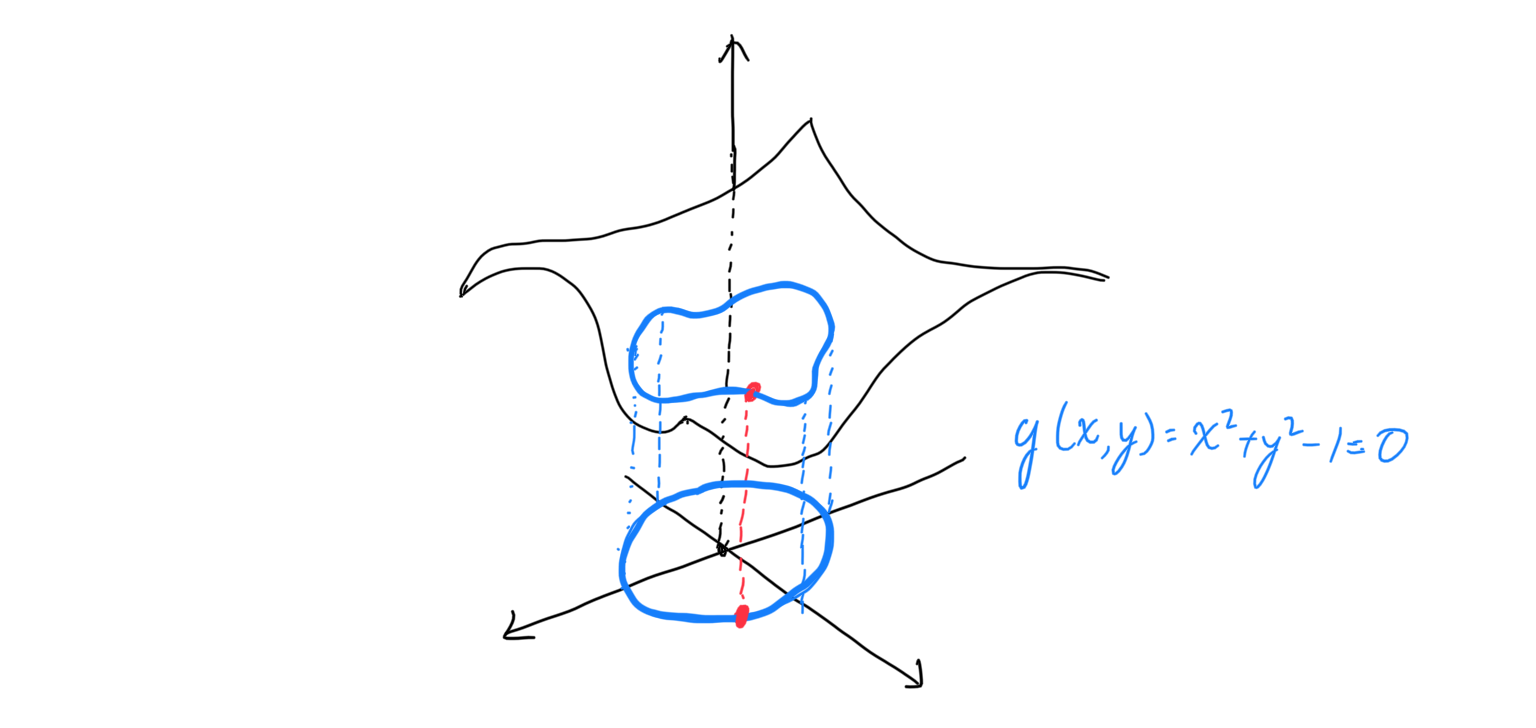
\includegraphics[scale=0.2]{img/Function_with_Constraints.PNG}
  \end{center}
  To solve this constraint problem, we use the method of Lagrange multipliers. The basic idea is to convert a constrained problem into a form such that the derivative test of an unconstrained problem can still be applied. The relationship between the gradient of the function and gradients of the constraints rather naturally leads to a reformulation of the original problem, known as the \textit{Lagrangian function}. That is, in order to find the maximum/minimum of $f$ subjected to the equality constraint $\mathbf{g}(\mathbf{x}) = \mathbf{0}$, we form the Lagrangian function
  \[\mathcal{L}(\mathbf{x}, \lambda) \equiv f(\mathbf{x}) - \boldsymbol{\lambda}^T \mathbf{g}(\mathbf{x})\]
  and find the stationary points of $\mathcal{L}$ considered as a function of $\mathbf{x} \in D$ and the Lagrange multiplier $\lambda \in \mathbb{R}$. The main advantage to this method is that it allows the optimization to be solved without explicit parameterization in terms of the constraints. 

  \begin{theorem}[Lagrange Multipliers Theorem]
  Let $f: \mathbb{R}^n \longrightarrow \mathbb{R}$ be a $C^1$ function and let $g(\mathbf{x}) = 0$, where $g: \mathbb{R}^n \longrightarrow \mathbb{R}^c$, be a system of $C^1$ constraint equations: $g \coloneqq (g_1, g_2, \ldots, g_c)$. Let $\mathbf{x}^*$ be an optimal solution to the optimization problem of maximizing $f(\mathbf{x})$ subject to the constraint $g(\mathbf{x}) = 0$ such that $\rank D g_{\mathbf{x}^*} = c < n$. Then, their exists a unique vector $\boldsymbol{\lambda}^*$ of Lagrange multipliers $\lambda_1^*, \lambda_2^*, \ldots, \lambda_c^*$ s.t. 
  \[D f_{\mathbf{x}^*} = \lambda^{*T} D g_{\mathbf{x}^*}\]
  where $D f_{\mathbf{x}^*}$ can be interpreted as the $1 \times n$ Jacobian matrix of $f$ and $D g_{\mathbf{x}^*}$ as the $c \times n$ Jacobian of $g$. Since both $D f_{\mathbf{x}^*}$ and $\lambda^{*T} D g_{\mathbf{x}^*}$ are maps from $\mathbb{R}^n$ to $\mathbb{R}$, we can invoke Riesz representation theorem to turn this into gradients: 
  \[\nabla f(\mathbf{x}^*) = \nabla \mathbf{g}(\mathbf{x}^*) (\boldsymbol{\lambda}^*)\]
  which has a matrix realization of 
  \begin{align*}
  \begin{pmatrix}
  \frac{\partial f}{\partial x_1} (\mathbf{x}^*) \\ \vdots\\ \frac{\partial f}{\partial x_n} (\mathbf{x}^*) \end{pmatrix} & = \begin{pmatrix}
  \frac{\partial g_1}{\partial x_1} (\mathbf{x}^*)& \ldots & \frac{\partial g_c}{\partial x_1} (\mathbf{x}^*)\\
  \vdots & \ddots & \vdots \\
  \frac{\partial g_1}{\partial x_n} (\mathbf{x}^*)& \ldots & \frac{\partial g_c}{\partial x_n}(\mathbf{x}^*)
  \end{pmatrix} \begin{pmatrix}
  \lambda^*_1 \\ \vdots \\ \lambda^*_c \end{pmatrix} \\
  & = \lambda^*_1 \begin{pmatrix}
  \frac{\partial g_1}{\partial x_1} (\mathbf{x}^*) \\ \vdots \\ \frac{\partial g_1}{\partial x_n}(\mathbf{x}^*)
  \end{pmatrix} + \lambda^*_2 \begin{pmatrix}
  \frac{\partial g_2}{\partial x_1} (\mathbf{x}^*) \\ \vdots \\ \frac{\partial g_2}{\partial x_n}(\mathbf{x}^*)
  \end{pmatrix} + \ldots + \lambda^*_c \begin{pmatrix}
  \frac{\partial g_c}{\partial x_1} (\mathbf{x}^*) \\ \vdots \\ \frac{\partial g_c}{\partial x_n}(\mathbf{x}^*)
  \end{pmatrix}
  \end{align*}
  This equation tells us that at any critical points $\mathbf{x}^*$ of $f$ evaluated under the equality constraints, the gradient of $f$ at $\mathbf{x}^*$ can be expressed as a unique linear combination of the gradients of the constraints $\nabla g_i (\mathbf{x}^*)$ (at $\mathbf{x}^*$), with the Lagrange multipliers acting as coefficients. Therefore, finding the critical points $\mathbf{x}^*$ of $f$ constrained with $g$ is equivalent to solving the system of $c + n$ equations for the $n$ unknowns in $\mathbf{x}$ and $c$ unknowns in $\boldsymbol{\lambda}$: 
  \begin{align*}
      \mathbf{g}(\mathbf{x}) & = 0 \\ 
      \nabla f(\mathbf{x}) & = \nabla \mathbf{g}(\mathbf{x}) (\boldsymbol{\lambda})
  \end{align*} 
  which can be rewritten as
  \begin{align*}
      c \text{ constraint equations} & \begin{cases}
      g_1 (x) & = 0 \\
      \ldots & = 0 \\
      g_c (x) & = 0
      \end{cases} \\
      n \text{ Lagranaian equations} & \begin{cases}
     \frac{\partial f}{\partial x_1} (\mathbf{x}^*) & = \lambda^*_1 \frac{\partial g_1}{\partial x_1} (\mathbf{x}^*) + \lambda^*_2 \frac{\partial g_2}{\partial x_1} (\mathbf{x}^*) + \ldots + \lambda^*_c \frac{\partial g_c}{\partial x_1} (\mathbf{x}^*) \\
      \ldots & = \ldots \\
      \frac{\partial f}{\partial x_n} (\mathbf{x}^*) & = \lambda^*_1 \frac{\partial g_1}{\partial x_n} (\mathbf{x}^*) + \lambda^*_2 \frac{\partial g_2}{\partial x_n} (\mathbf{x}^*) + \ldots + \lambda^*_c \frac{\partial g_c}{\partial x_n} (\mathbf{x}^*) 
      \end{cases}
  \end{align*}
  \end{theorem}

  More abstractly, $D f_{\mathbf{x}^*}$ is the linear functional in $(\mathbb{R}^n)^*$, and $D g_{\mathbf{x}^*}$, which is a linear map from $\mathbb{R}^n$ to $\mathbb{R}^c$, can be interpreted as a map from $(\mathbb{R}^c)^*$ to $(\mathbb{R}^n)^*$ Since $\boldsymbol{\lambda}^*$ "lives" in $(\mathbb{R}^c)^*$, $D g_{\mathbf{x}^*}(\boldsymbol{\lambda}^*) \in (\mathbb{R}^n)^*$, which is the same space that $f_{\mathbf{x}^*}$ lives in. 


  Let us introduce a visualization for when where is a single constraint $g: \mathbb{R}^n \longrightarrow \mathbb{R}$. From the properties of the gradient, $\nabla f(x_0)$ is orthogonal to the level set of points satisfying $f(x) = f(x_0)$ at point $x_0$. Note that the constraint function $g$ also maps $\mathbb{R}^n \longrightarrow \mathbb{R}$, and so it has its own level surfaces. We can see that the point where the contour line of $g(x) = 0$ tangentially touches the contours of $f$ is the maximum. Since it intersects it tangentially, the gradient vector at that point $\nabla g(x_0)$ is parallel to $\nabla f(x_0)$. 
  \begin{center}
      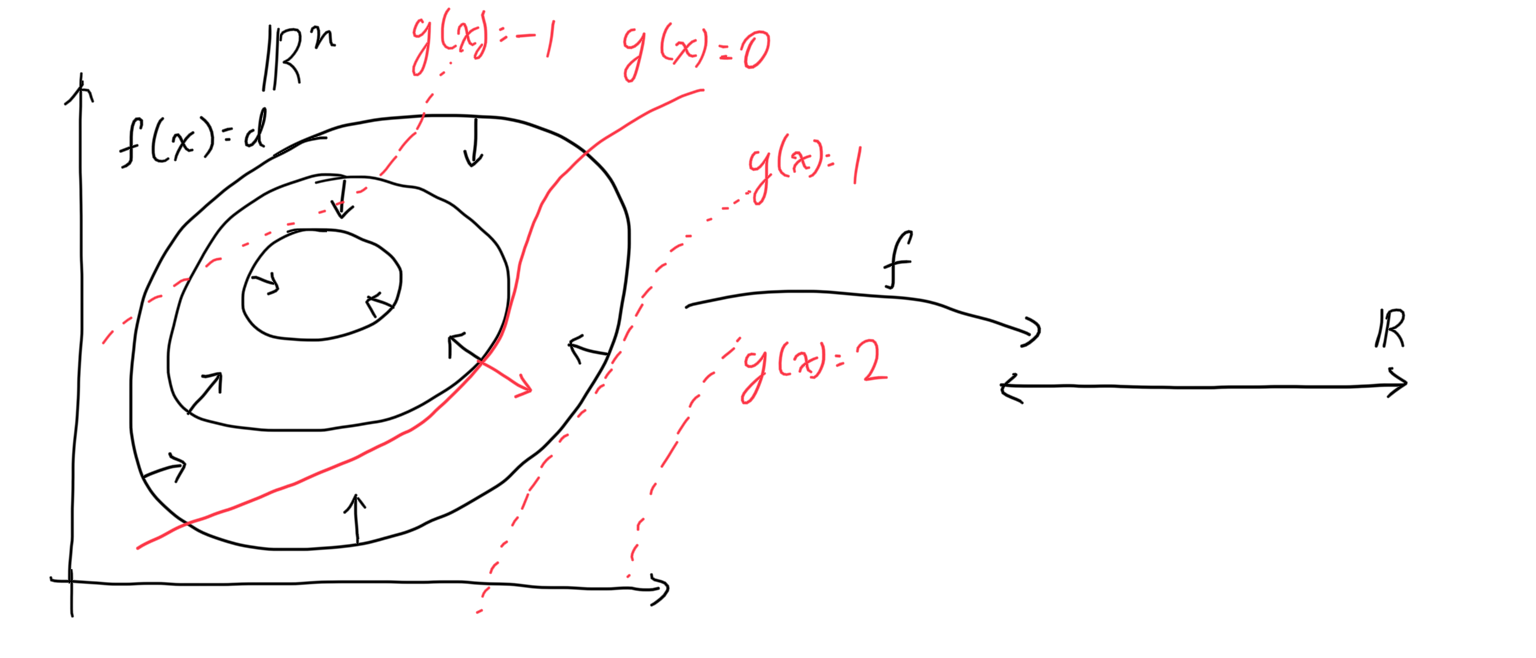
\includegraphics[scale=0.22]{img/Lagrange_Multiplier_Single_Constraint.PNG}
  \end{center}
  We can visualize this for multiple constraints as well, where $\nabla f(x_0)$ (the gradient vector of $f$ at $x^*$) can be expressed as a linear combination of $\nabla g_1 (x_0)$ and $\nabla g_2 (x_0)$ (gradient vectors of the constraint functions at $x^*$). 
  \begin{center}
      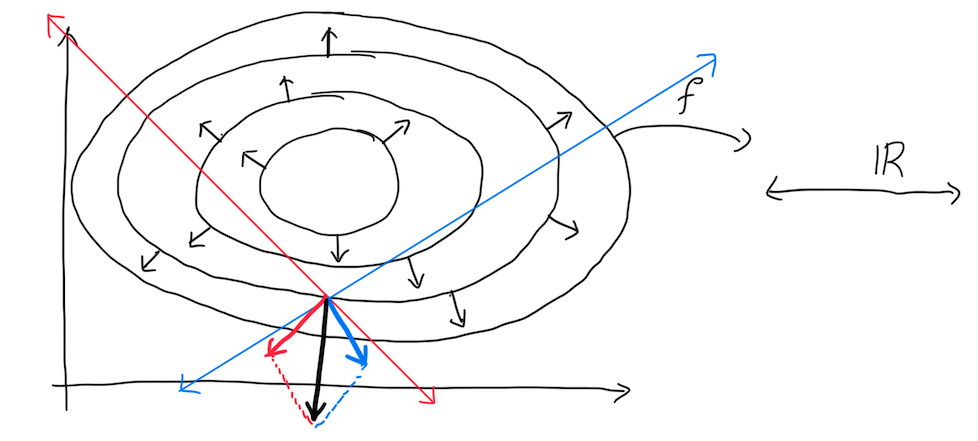
\includegraphics[scale=0.27]{img/Lagrange_Multiplier_Multiple_Constraints.PNG}
  \end{center}

  From the properties of the gradient introduced before, $\triangledown f(x_0)$ is orthogonal to the level set of points satisfying $f(x) = c$ at the point $x_0$. But this level set $f(x) = c$ actually intersects the level set determined by $g(x) = c$ at the point $x_0$ and is indistinguishable from each other at $x_0$. This means that $\triangledown g(x_0)$ is normal the level set of $g(x) = c$ at $x_0 \iff $ it is normal to the level set of $f(x) = c$ at $x_0$. But $\triangledown f(x_0)$ is also normal at that point, so $\triangledown f(x_0)$ must be parallel to $\triangledown g(x_0)$. 

\subsection{Inverse and Implicit Function Theorems} 

  \begin{theorem}[Inverse Function Theorem for Multivariable Functions and its Matrix Realization]
  Let $\mathbf{f}: \mathbb{R}^n \longrightarrow \mathbb{R}^n$ be a $C^1$ function defined on an open neighborhood of $\mathbf{x}_0$ in the domain. If the total derivative/Jacobian $D \mathbf{f}_{\mathbf{x}_0}$ at $\mathbf{x}_0$ is invertible, an inverse function of $\mathbf{f}$ is defined on some neighborhood of $\mathbf{y}_0 = \mathbf{f}(\mathbf{x}_0)$. Given that we are working with a fixed basis, $\mathbf{f}$ can be modeled by the set of $n$ equations 
  \begin{align*}
      f_1 (x_1, x_2, \ldots, x_n) &= y_1 \\
      \ldots & = \ldots \\
      f_2 (x_1, x_2, \ldots, x_n) &= y_2
  \end{align*}
  This theorem says that this system of $n$ equations has a unique solution for $x_1, x_2, \ldots, x_n$ in terms of $y_1, \ldots, y_n$, provided that we restrict $\mathbf{x}$ and $\mathbf{y}$ to small enough neighborhoods of $\mathbf{x}_0$ and $\mathbf{y}_0$. This inverse function $\mathbf{f}^{-1}: \mathbb{R}^n \longrightarrow \mathbb{R}^n$ is also $C^1$, and its total derivative/Jacobian $D \mathbf{f}^{-1}_{\mathbf{y}_0}$ at $\mathbf{y}_0 = \mathbf{f}(\mathbf{x}_0)$ is the inverse linear map of $D \mathbf{f}_{\mathbf{y}_0}$. 
  \[D \mathbf{f}^{-1}_{\mathbf{y}_0} = \big( D \mathbf{f}_{\mathbf{x}_0} \big)^{-1}\]
  \end{theorem}

  \begin{example}
  Consider the vector-valued function $\mathbf{f}: \mathbb{R}^2 \longrightarrow \mathbb{R}^2$ defined by 
  \[\mathbf{f}(x_1, x_2) = \begin{pmatrix}
  e^{x_1}\cos (x_2) \\ e^{x_1} \sin(x_2)
  \end{pmatrix}\]
  The total derivative/Jacobian matrix is 
  \[J \mathbf{f}(x_1, x_2) = \begin{pmatrix}
  e^{x_1} \cos(x_2) & - e^{x_1} \sin(x_2) \\
  e^{x_1} \sin(x_2) & e^{x_1} \cos(x_2)
  \end{pmatrix} \implies \det J \mathbf{f}(x_1, x_2) = e^{2x_1} \cos^2 (x_2) + e^{2x_1} \sin^2 (x_2) = e^{2x_1}\]
  Since the determinant $e^{2x_1}$ is nonzero everywhere, $D \mathbf{f}_\mathbf{x}$ is nonsingular. Thus, the theorem guarantees that for every point $\mathbf{x}_0 \in \mathbb{R}^2$, there exists a neighborhood about $\mathbf{x}_0$ over which $\mathbf{f}$ is invertible. However, this does not mean $\mathbf{f}$ is invertible over its entire domain: in this case $\mathbf{f}$ isn't even injective since it is periodic: e.g. the preimage of $(e, 0)$ contains $(1, 0)$ and $(1, 2\pi)$. 
  \end{example}

  Remember that given an explicit representation of a set $\mathbf{y} = \mathbf{f}(\mathbf{x})$, we can easily find the implicit form as $\mathbf{F}(\mathbf{x}, \mathbf{y}) = \mathbf{y} - \mathbf{f}(\mathbf{x}) = \mathbf{0}$. What about the other way around? That is, given an implicit representation of some surface, what conditions must be met so that it can be represented as the graph of a function? The implicit function theorem is a tool that allows relations between points in $\mathbb{R}^n$ to be converted to functions of several real variables. That is, it states that for sufficiently "nice" points on a $n$-dimensional surface defined as $\mathbf{F}(\mathbf{x}, \mathbf{y}) = \mathbf{0}$ (where $\mathbf{F}: \mathbb{R}^{n+m} \longrightarrow \mathbb{R}^m$), we can locally pretend that this surface is a graph of a function $\mathbf{g}: \mathbb{R}^n \longrightarrow \mathbb{R}^m$ whose graph $\big(\mathbf{x}, \mathbf{g}(\mathbf{x})\big)$ is precisely the set of all $(\mathbf{x}, \mathbf{y})$ s.t. $\mathbf{f}(\mathbf{x}, \mathbf{y}) = \mathbf{0}$. When $m = 1$, it basically states that if an implicit surface suffices the vertical line test in a neighborhood, then it can be written as a function. 

  \begin{example}[Circle]
    Let $f: \mathbb{R}^2 \longrightarrow \mathbb{R}$ be defined by $f(x, y) = x^2 + y^2 - 1$. The level set at $z = 0$ would be the set of points satisfying 
    \[x^2 + y^2 - 1 = 0\]
    the unit circle. The derivative of $f$ with respect to $y$ is $0$ at the points $(-1,0)$ and $(1,0)$, meaning that in any neighborhood of these points, we cannot define a function of $y$ with respect to $x$. This is true, indeed, since any such function would fail the vertical line test, which can be seen in the red neighborhood around $(1,0)$. However, the blue neighborhood of the point $(-\sqrt{2}/2, \sqrt{2}/2)$ does indeed define a function of $y$ with respect to $x$ satisfying the vertical line test. 
    \begin{center}
    \begin{tikzpicture}
      \draw[<->] (-3,0)--(3,0);
      \draw[<->] (0,-3)--(0,3);
      \draw (0,0) circle (2);
      \draw[fill=red] (2,0) circle (0.08);
      \draw[fill=red] (-2,0) circle (0.08);
      \draw[red, thick] (1.732, -1) arc (-30:60:2);
      \draw[dashed, <->] (1.8,-2.5)--(1.8,2.5);
      \draw[fill=blue] (-1.414, 1.414) circle (0.08);
      \draw[blue, thick] (-1, 1.732) arc (120:170:2);
      \draw[dashed,<->] (-1.7,2.5)--(-1.7,-2.5);
    \end{tikzpicture}
    \end{center}
  \end{example}

  \begin{theorem}[Special Implicit Function Theorem]
    Let $f: \mathbb{R}^{n+1} \longrightarrow \mathbb{R}$ be a $C^1$ function with a point $(a, b) \in \mathbb{R}^{n+1}$ on the level set $f(\mathbf{x}, y) = 0$. If $\partial_y f (a, b)$, which can also be thought of as the $1 \times 1$ truncated Jacobian matrix $D_\mathbf{y} f_{(a, b)} = \partial_{y} f(a, b)$ w.r.t. $y$, of 
    \[D f_{(a, b)} = \begin{pmatrix} D_\mathbf{x} f_{(a, b)} & D_\mathbf{y} f_{(a, b)} \end{pmatrix} = \left(\begin{array}{ccc|c}
       \partial_{x_1} f(a, b) &\ldots & \partial_{x_n} f(a, b) & \partial_{y} f(a, b)
       \end{array}\right)\]
    is invertible (in this case nonzero), then there exists an open neighborhood $U_a \subset \mathbb{R}^n$ of $a$ and a unique $C^1$ function $y: U \subset \mathbb{R}^n \longrightarrow \mathbb{R}$ s.t. $f\big(\mathbf{x}, y(\mathbf{x})\big) = 0$ for all $\mathbf{x} \in U$. That is, we can find a $y: U \longrightarrow \mathbb{R}$ s.t. the graph $y(\mathbf{x})$ within $U$ coincides with the graph of $f(\mathbf{x}, y) = 0$. Moreover, the total derivative/Jacobian of $y: \mathbb{R}^n \longrightarrow \mathbb{R}$ in $U$ is the $1 \times n$ matrix given by the matrix product
    \[D g_a = - (D_y f_a)^{-1} D_\mathbf{x} f_a\]
  \end{theorem}

  \begin{example}[Circle Example]
    Let $n = m = 1$ and $f(x_1, x_2) = x_1^2 + x_2^2 - 1$. We would like to find out at which points $a$ can this surface be explicitly represented by a function $g: U_a \subset \mathbb{R} \longrightarrow \mathbb{R}$ defining $x_2$ from $x_1$. Its Jacobian is 
    \[D f = \begin{pmatrix} \partial_{x_1} f & \partial_{x_2} f \end{pmatrix} = \begin{pmatrix} 2 x_1 & 2x_2 \end{pmatrix} \]
    The truncated Jacobian w.r.t. $x_2$ is $2 x_2$, which is invertible iff $x_2 \neq 0$. By the implicit function theorem, we can locally write the circle in the form $x_2 = g(x_1)$ for all points where $x_2 \neq 0$. This is easy to see. For example, we can choose the point $(0.8, 0.6)$ on the level set, and the appropriate explicit function is 
    \[x_2 = g(x_1) = \sqrt{1 - x_1^2}\]
    within the neighborhood of $x_1 = 0.8$. For $(\pm 1, 0)$, we cannot since every function defined within a neighborhood of $x_1 = \pm 1$ fails the vertical line test. The derivative of $g$, by the theorem, can be defined implicitly as 
    \[D g = - ( \partial_{x_2} f)^{-1} D_{x_1} f = - (2 x_2)^{-1} (2 x_1) = -\frac{x_1}{x_2}\]
    which leads to the differential equation 
    \[g^\prime (x_1) = - \frac{x_1}{g(x_1)} \text{ where we solve for } g\]
    If we would have liked to find a function $h: U_{a_{\mathbf{x}_2}} \subset \mathbb{R} \longrightarrow \mathbb{R}$ defining $x_1$ from $x_2$, then we can redo everything to find that the truncated Jacobian w.r.t. $x_1$ is $2x_1$, which is invertible iff $x_1 \neq 0$, and the the derivative is 
    \[D h = - (\partial_{x_1} f)^{-1} D_{x_2} f = - (2x_1)^{-1} (2x_2) = -\frac{x_2}{x_1}\]
    which leads to the differential equation 
    \[h^\prime (x_2) = - \frac{x_2}{h(x_2)} \text{ where we solve for } h\]
  \end{example}

  \begin{theorem}[General Implicit Function Theorem]
    Let $f: \mathbb{R}^{n+m} \longrightarrow \mathbb{R}^m$ be a $C^1$ function with a point $(a, \mathbf{b}) \in \mathbb{R}^{n + m}$ on the level set $f( \mathbf{x}, \mathbf{y}) = 0$. If the $m \times m$ truncated Jacobian matrix $D_{\mathbf{y}} f (a, \mathbf{b})$ w.r.t. $\mathbf{y}$, of 
    \[D f_{(a, \mathbf{b})} = \begin{pmatrix} D_\mathbf{x} f_{(a, \mathbf{b})} & D_\mathbf{y} f_{(a, \mathbf{b})} \end{pmatrix}\]
    is invertible, then there exists an open neighborhood $U_a \subset \mathbb{R}^n$ of $a$ and a unique $C^1$ function $\mathbf{y}: U \subset \mathbb{R}^n \longrightarrow \mathbb{R}^m$ s.t. $f\big(\mathbf{x}, \mathbf{y}(\mathbf{x}) \big) = 0$ for all $\mathbf{x} \in U$. That is, we can find a $\mathbf{y}: U \longrightarrow \mathbb{R}^m$ s.t. the graph $\mathbf{y}(\mathbf{x})$ within $U$ coincides with the graph of $f(\mathbf{x}, \mathbf{y}) = 0$. Moreover, the total derivative/Jacobian of $\mathbf{y}$ is the $m \times n$ matrix given by the matrix product 
    \[D g_a = - (D_\mathbf{y} f_a)^{-1} D_\mathbf{x} f_a\]
  \end{theorem}

